\section{Sesión 6}


\begin{teorema}
	Suponga que $f,g:[a,b]\to\mathbb{R}$, funciones acotadas y tales que $f(x)=g(x)$, excepto en un número finito de puntos $x\in[a,b]$. Entonces $f\in R[a,b]$ ssi $g\in R[a,b]$, y se tiene que: 
	
	$$\int_a^b f=\int_a^b g.$$
\end{teorema}


\begin{prop}
	Suponga que $f:[a,b]\to\mathbb{R}$ es acotada e integrable en $[a,r]$, para cada $a<r<b$. Entonces, $f$ es integrable en $[a,b]$ y se tiene: 
	$$\int_a^b=\lim_{r\to b^-}\int_a^r f.$$
\end{prop}
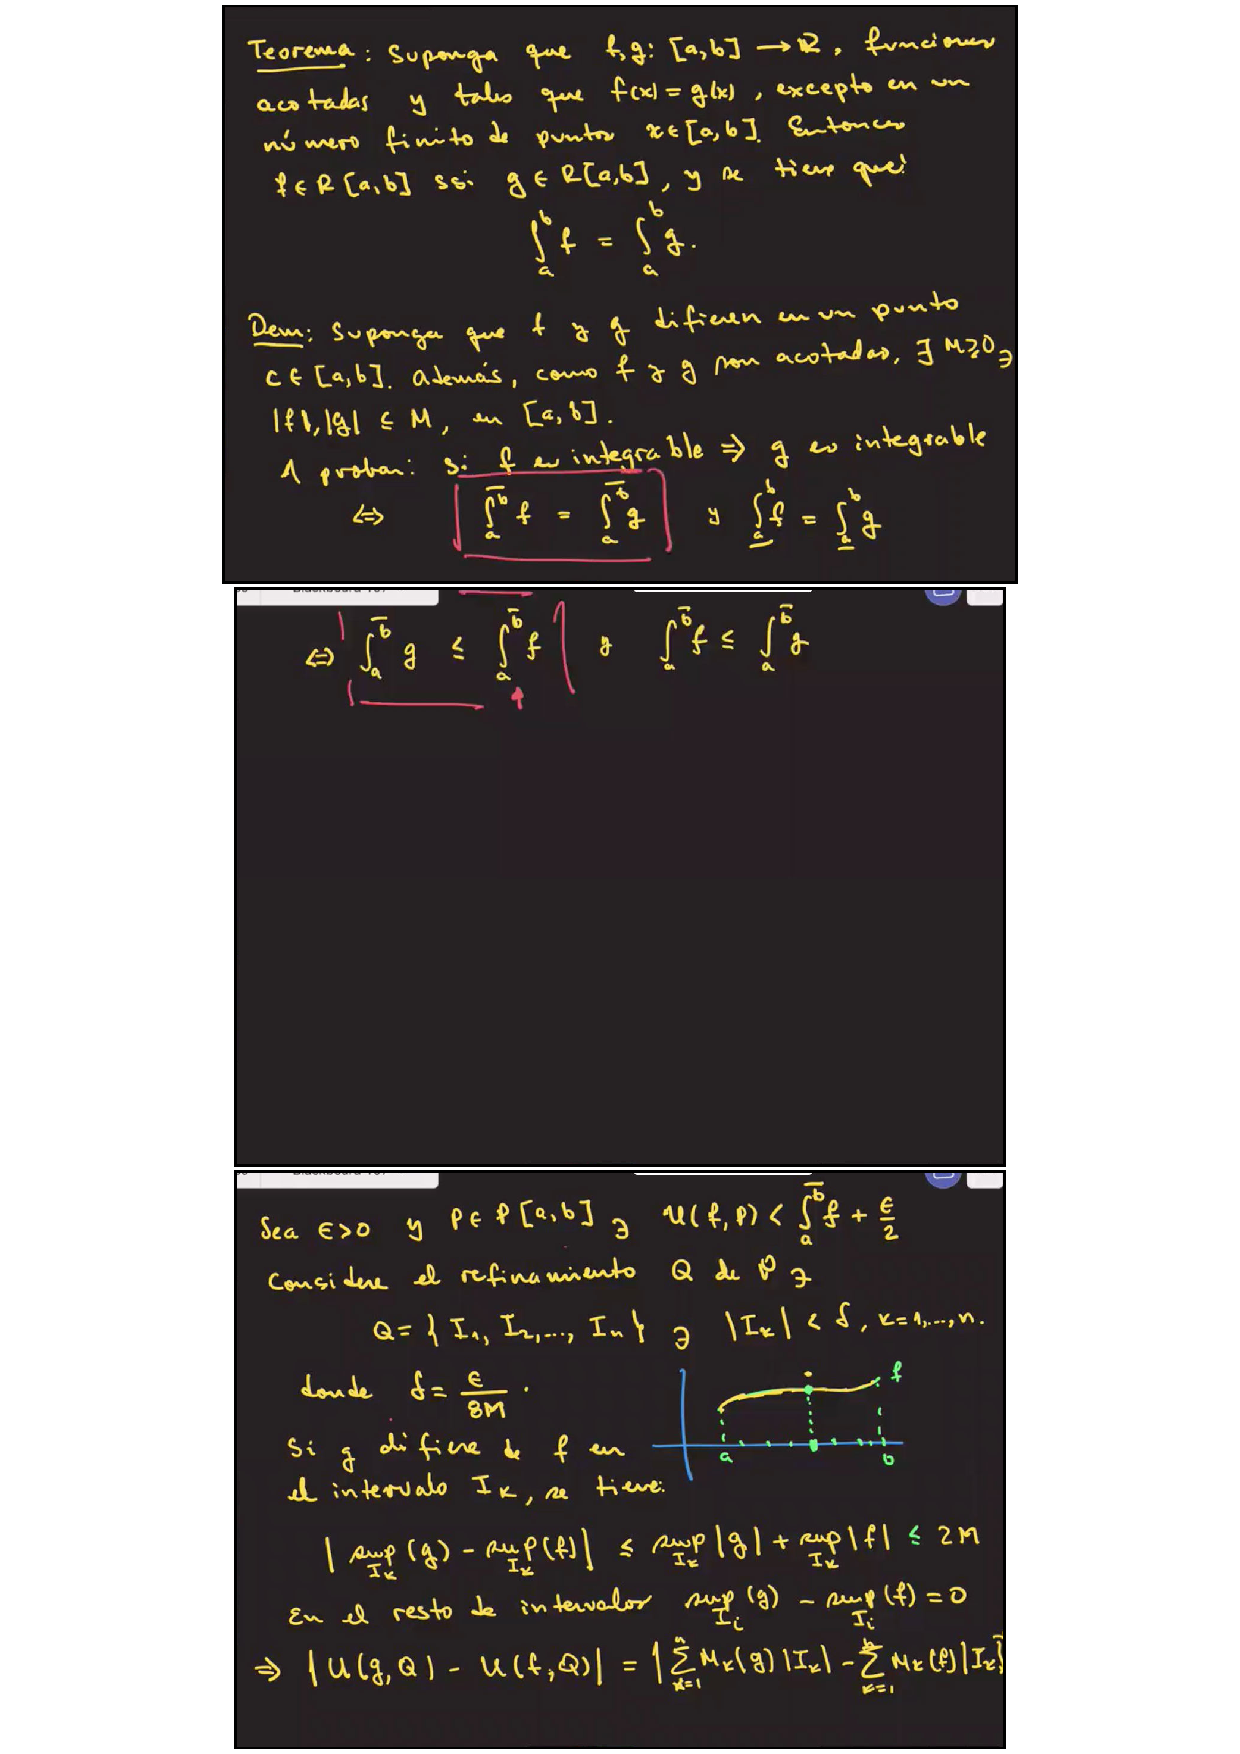
\includepdf[pages=-]{apendices/s6.pdf}